\documentclass{beamer}
\usefonttheme[onlymath]{serif}
\usepackage[T1]{fontenc}
\usepackage[utf8]{inputenc}
\usepackage[english]{babel}
\usepackage{amsmath}
\usepackage{amssymb}
\usepackage{amsthm}
\usepackage{gensymb}
\usepackage{parskip}
\usepackage{mathtools}
\usepackage{listings}
\usepackage{hyperref}
\usepackage{graphicx}
\usepackage{color}
\usepackage{enumerate}
\usepackage{tikz}
\usetikzlibrary{calc}
\usetikzlibrary{positioning}
\usetikzlibrary{angles}
\usetikzlibrary{shapes}
\usetikzlibrary{arrows}
\usepackage{verbatim}
\usepackage{multicol}
\usepackage{array}
\usepackage{minted}
\parskip 0pt


\DeclareMathOperator{\lcm}{lcm}
\newcommand\floor[1]{\left\lfloor#1\right\rfloor}
\newcommand\ceil[1]{\left\lceil#1\right\rceil}
\newcommand\abs[1]{\left|#1\right|}
\newcommand\p[1]{\left(#1\right)}
\newcommand\sqp[1]{\left[#1\right]}
\newcommand\cp[1]{\left\{#1\right\}}
\newcommand\norm[1]{\left\lVert#1\right\rVert}
\renewcommand\Im{\operatorname{Im}}
\renewcommand\Re{\operatorname{Re}}

\usetheme{metropolis}
\definecolor{dark yellow}{rgb} {0.6,0.6,0.0}
\definecolor{dark green}{rgb} {0.0,0.6,0.0}

\graphicspath{{myndir/}}

\title{Sparse Table / Binary Lifting}
\author{Arnar Bjarni Arnarson}
\institute{\href{http://ru.is/td}{School of Computer Science} \\[2pt] \href{http://ru.is}{Reykjavík University}}
\titlegraphic{\hfill
\includegraphics[height=0.6cm]{kattis}}

\begin{document}
\maketitle

\begin{frame}[plain]{Range queries}
    \vspace{30pt}
    \begin{itemize}
        \item<1-> We have an array $A$ of size $n$.
        \item<2-> Given $i,j$, we want to answer:
            \begin{itemize}
                \item<3-> $\mathrm{max}(A[i],A[i+1],\ldots,A[j-1],A[j])$
                \item<4-> $\mathrm{min}(A[i],A[i+1],\ldots,A[j-1],A[j])$
                \item<5-> $\mathrm{sum}(A[i],A[i+1],\ldots,A[j-1],A[j])$
            \end{itemize}
        \item<6-> We want to answer these queries efficiently, or in other words, without looking through all elements.
        \item<7-> Sometimes we also want to update elements.
    \end{itemize}
\end{frame}

\begin{frame}[plain]{Another $\log(n)$ idea}
    \begin{itemize}
        \item<1-> What if we tried something more akin to an array.
        \item<2-> Could we store $\log(n)$ amounts of data per element somehow?
        \item<3-> Yes! For each $i$ we can store the sum on the interval $[i, i + 2^j - 1]$ for $\log$ many $j$.
        \item<4-> Then to retrieve a sum from $i$ to $j$ we always take the biggest chunk we can that's stored at $i$, which will always be at least half.
        \item<5-> Then we continue until we reach $j$, moving $i$ along and collecting the results.
        \item<6-> This is what is known as a sparse table.
    \end{itemize}
\end{frame}

\begin{frame}[plain]{Sparse tables}
    \begin{itemize}
        \item<1-> Calculating all of these values takes $\mathcal{O}(n\log(n))$ because we can calculate the values in order of increasing $j$.
        \item<2-> Then when we calculate the sum of $[i, i + 2^j - 1]$ we just combine the earlier results of $[i, i + 2^{j-1} - 1]$ and $[i + 2^{j-1}, i + 2^j - 1]$.
        \item<3-> Querying takes $\mathcal{O}(\log(n))$, however updating is slow and difficult.
        \item<4-> Why would we then ever use this instead of segment trees?
    \end{itemize}
\end{frame}

\begin{frame}[plain]{Binary lifting}
    \begin{itemize}
        \item<1-> The reason might be is that with sparse tables we can do many things that segment trees can not because of how the results are combined.
        \item<2-> Let us consider binary lifting in particular.
        \item<3-> Suppose we have some function $f$ that rearranges the values $\{0, 1, \dots, n - 1\}$ and we get $q$ queries asking what happens to $x$ if we apply $f$ exactly $m$ times to $x$.
        \item<4-> The naïve solution is to calculate it every time, giving a time complexity of $\mathcal{O}(qm\mathcal{O}(f))$.
        \item<5-> How might we use sparse tables to do better?
    \end{itemize}
\end{frame}

\begin{frame}[plain]{Binary lifting ctd.}
    \begin{itemize}
        \item<1-> Let $f^{[y]}(x)$ denote the result of applying $f$ exactly $y$ times to $x$
        \item<2-> For each $i$ we store $f^{[2^j]}(i)$ as a sparse table
        \item<3-> Then we can compute these in increasing order of $j$, calculating $j = 1$ using $f$ itself and then for larger $j$ letting $f^{[2^j]}(x) = f^{[2^{j-1}]}(f^{[2^{j-1}]}(x))$
        \item<4-> Thus we can precompute the table in $\mathcal{O}(n(\mathcal{O}(f) + \log(n)))$ and each query takes $\mathcal{O}(\log(m))$, a much better time complexity
    \end{itemize}
\end{frame}

\begin{frame}[plain]{Sparse table example}
    \begin{center}
        \begin{tikzpicture}[scale=0.75]
            \draw[step=1,black,thin] (0,0) grid (12, 1);
            \node[align=left] at (13.5,0.5) {$j = 0$};
            \node at (0.5,0.5) {$7$};
            \node at (1.5,0.5) {$1$};
            \node at (2.5,0.5) {$6$};
            \node at (3.5,0.5) {$4$};
            \node at (4.5,0.5) {$8$};
            \node at (5.5,0.5) {$0$};
            \node at (6.5,0.5) {$9$};
            \node at (7.5,0.5) {$2$};
            \node at (8.5,0.5) {$2$};
            \node at (9.5,0.5) {$7$};
            \node at (10.5,0.5) {$1$};
            \node at (11.5,0.5) {$6$};

            \only<2-> {
                \draw[step=1,blue,thin] (0,1) grid (12, 2);
                \node[align=left] at (13.5,1.5) {\color{blue} $j = 1$};
            }
            \foreach \x in {3,4,...,13} {
                \only<\x> {
                    \draw[->, blue] ({0.5+\x-3}, 0.75) -- ({0.5+\x-3}, 1.25);
                    \draw[->, blue] ({1.25+\x-3}, 0.75) -- ({0.75+\x-3}, 1.25); 
                }
            }
            \foreach \x [count=\i] in {8, 7, 10, 12, 8, 9, 11, 4, 9, 8, 7, 6} {
                \pgfmathtruncatemacro{\onlyi}{\i+2}
                \only<\onlyi-> {
                    \node at ({-0.5+\i},1.5) {\color{blue} $\x$};
                }
            }

            \only<14> {
                \draw[->, blue] (11.5, 0.75) -- (11.5, 1.25);
            }

            \only<15-> {
                \draw[step=1,dark green,thin] (0,2) grid (12, 3);
                \node[align=left] at (13.5,2.5) {\color{dark green} $j = 2$};
            }
            \foreach \x in {3,4,...,12} {
                \only<15> {
                    \draw[->, dark green] ({0.5+\x-3}, 1.75) -- ({0.5+\x-3}, 2.25);
                    \draw[->, dark green] ({1.25+\x-2}, 1.75) -- ({0.75+\x-3}, 2.25); 
                }
            }
            \only<15> {
                \draw[->, dark green] (11.5, 1.75) -- (11.5, 2.25);
                \draw[->, dark green] (10.5, 1.75) -- (10.5, 2.25);
            }
            \foreach \x [count=\i] in {18, 19, 18, 21, 19, 13, 20, 12, 16, 14, 7, 6} {
                \only<15-> {
                    \node at ({-0.5+\i},2.5) {\color{dark green} $\x$};
                }
            }

            \only<16-> {
                \draw[step=1,dark yellow,thin] (0,3) grid (12, 4);
                \node[align=left] at (13.5,3.5) {\color{dark yellow} $j = 3$};
            }
            \foreach \x in {3,4,...,10} {
                \only<16> {
                    \draw[->, dark yellow] ({0.5+\x-3}, 2.75) -- ({0.5+\x-3}, 3.25);
                    \draw[->, dark yellow] ({1.25+\x}, 2.75) -- ({0.75+\x-3}, 3.25); 
                }
            }
            \only<16> {
                \draw[->, dark yellow] (11.5, 2.75) -- (11.5, 3.25);
                \draw[->, dark yellow] (10.5, 2.75) -- (10.5, 3.25);
                \draw[->, dark yellow] (9.5, 2.75) -- (9.5, 3.25);
                \draw[->, dark yellow] (8.5, 2.75) -- (8.5, 3.25);
            }
            \foreach \x [count=\i] in {37, 32, 38, 33, 35, 27, 27, 18, 16, 14, 7, 6} {
                \only<16-> {
                    \node at ({-0.5+\i},3.5) {\color{dark yellow} $\x$};
                }
            }

            \only<17> {
                \node at (5, 5) {\texttt{query(1, 8) = 19 + 9 + 2}};
                \draw[red, very thick] (1, 2) -- (2, 2) -- (2, 3) -- (1, 3) -- cycle;
                \draw[red, very thick] (5, 1) -- (6, 1) -- (6, 2) -- (5, 2) -- cycle;

                \draw[red, very thick] (1, 0) -- (5, 0) -- (5, 1) -- (1, 1) -- cycle;
                \draw[red, very thick] (5, 0) -- (7, 0) -- (7, 1) -- (5, 1) -- cycle;
                \draw[red, very thick] (7, 0) -- (8, 0) -- (8, 1) -- (7, 1) -- cycle;
            }

            \only<18> {
                \node at (5, 5) {\texttt{query(0, 9) = 37 + 9}};
                \draw[red, very thick] (0, 3) -- (1, 3) -- (1, 4) -- (0, 4) -- cycle;
                \draw[red, very thick] (8, 1) -- (9, 1) -- (9, 2) -- (8, 2) -- cycle;

                \draw[red, very thick] (0, 0) -- (8, 0) -- (8, 1) -- (0, 1) -- cycle;
                \draw[red, very thick] (8, 0) -- (10, 0) -- (10, 1) -- (8, 1) -- cycle;
            }

        \end{tikzpicture}
    \end{center}
\end{frame}

\begin{frame}[plain]{Example problem: Stikl}
    \begin{itemize}
        \item https://open.kattis.com/problems/stikl
    \end{itemize}
\end{frame}

\end{document}
